\chapter{Introduction}
\inspirationalquote{
\begin{tabular}{p{0.7\textwidth}}
Please hold on. This thesis will be departing shortly for the Landslide terminal, baggage claim, ground transportation, and ticketing.
\end{tabular}}
{Pittsburgh International Airport (paraphrased)}

\revision{Pick up any recent concurrency-related research paper, %from the last few decades,
and chances are its very first sentence will tell you
%how notoriously difficult concurrency bugs are compared to sequential ones
that concurrency bugs are notoriously difficult to find, reproduce, diagnose, and/or fix
% ,
%and/or thereafter verify fixed,
%compared to sequential ones,
%on account of the multitude of thread interleavings one must test
\cite{nidhugg,optimal-dpor,coredet,sealing,quicksand,landslide,this-thesis,concuerror,
%cspec, % 2nd sentence in cspec >_>
bpor,
%parrot, % 2nd sentence in parrot
peregrine,
%bugtm, % 1st and 2nd sentence
satcheck,
racerx,
%ifrit, % 1st para, approx
datacollider,
fasttrack,
mcr-tsopso,
mcr,
macemc,
contessa,
%lvish, % "it must become easier"
dthreads,
taxdc,
%learning-from-mistakes, % sentence 3ish
avio,
symbiosis,
chess-icb,
chess,
recordreplaydrs,
kendo, % first WHOLE PARAGRAPH geez dude
%hybriddatarace, % 3rd sentence
parallel-dpor,
%eraser, % 3rd sentence 2nd paragraph
%racefuzzer, % 2nd sentence
%tsan, % 2nd sentence
sully-thesis,
%compcerttso, % 2nd sentence
modist,
maple,
simtester}.
%compared to sequential programming.
%
%Indeed, just as conditional statements and loops introduce additional possible program behaviours
%depending on different input,
%concurrent execution introduces additional possible behaviours even under a fixed input.
%Unlike input nondeterminism,
%concurrency nondeterminism typically manifests at the whims of chance,
%making bug-finding and verification especially challenging.
%
%What is a concurrency bug, and
How could a single programming technique be so troublesome
as to inspire multiple decades of verification research?
Allow me to begin this thesis by answering this question
in layperson's terms,
using two parables.

My favourite way to explain concurrency to a non-technical audience
%(e.g., family members)
is by analogy with unlocking car doors.
In many %makes and
models of cars, the door handle and locking mechanism are intertwined
in such a way that the door cannot unlock while its handle is being pulled~\cite{car-doors}.
Most car users, then,
%are familiar with
have suffered the experience of
trying to open the passenger door
at exactly the same moment as the driver turns the key in the lock:
%not only does the door not open, but
it fails to unlock, and
they must beseech the driver to turn the key again!
If they had pulled the handle any later, it would have opened as normal;
any earlier, and it would have been as though not having the key at all,
but would at least have unlocked properly at the first turn of the key later.
One would reasonably expect to never have to turn the key more than once,
so this violation of expected behaviour is a {\em bug},
% more ambiguous version pointed out by garth
%This violation of expected behaviour -- that the key need not be turned twice -- is a {\em bug},
and its dependence on the two travelers' actions {\em interleaving}
%with the driver's actions
in a particular way
makes it a {\em concurrency bug}.
This example involves only three events (pulling the handle, releasing the handle, and turning the key),
but what of a system with hundreds or thousands of times more?
Unfortunately, the number of possible interleavings grows {\em exponentially} with the number of events.

%Exponential explosion is easily understood through the tale of Sissa Ibn D\`{a}hir
The Islamic historian Ibn Khallik\={a}n told perhaps the first cautionary tale of exponential explosion
\cite{ibn-khallikan,khallikān1868ibn}.
Sissa Ibn D\`{a}hir,
credited with the invention of chaturanga (the precursor to modern chess),
was invited by King Shihr\^{a}m to request any reward he desired.
Sissa requested that a grain of wheat be placed on the first square of a chessboard,
two in the second, and so on, doubling the number of grains in each previous square until all 64 be filled.
The king at first laughed, thinking it a pittance,
realizing only later that to fulfill this would require
more than all the wheat in all the cities on Earth.
Modern programmers will recognize this sum as $2^{64}$-$1$,
the largest value representable by an unsigned 64-bit integer,
or approximately 18 billion billion.
The number of interleavings in a concurrent system grows at a similarly intractable rate
(although not necessarily exactly doubling each time),
with the number of chessboard squares filled with grain corresponding to the number of events in a program's execution.
A concurrency bug, then, is a single poisoned grain of wheat,
which must be rooted out from the stock before feeding the townspeople.
And Sissa himself is the programmer,
whose software is invariably large enough to be far beyond the reach of any exhaustive verification strategy.
}

\section{Motivation}

To take advantage of multiple cores for performance, programmers must write software to execute concurrently,
i.e.,
using multiple threads to run several parts of a program's logic simultaneously.
However, when threads access the same shared data,
they may interleave in unexpected ways which change the outcome of their execution,
\revisionminor{just as when multiple travelers interact with car doors at the same time.}
When an unexpected interleaving produces undesirable program behaviour,
for example, by corrupting shared data structures,
\revisionminor{or by leaving the door locked as in the car example,}
we call it a {\em concurrency bug}.
\revisionminor{The specific interleaving required to expose such a bug}
arises at random during normal execution,
and often with very low probability.
%
Most commonly, a programmer searches for concurrency bugs in her code by running it many times (in parallel, in serial, or both),
hoping that eventually,
\revisionminor{she will chance upon such an interleaving should one exist.}
%it will run according to the particular interleaving required to expose a hypothetical bug.
This technique, known as {\em stress testing}, is unreliable,
providing no guarantee of finding the failing interleaving in any finite amount of time.
It also provides no assurance of correctness:
when finished, there is no way of knowing how many distinct thread interleavings were actually tested.
Nevertheless, stress testing remains popular because of how easily a programmer can use it:
she simply wraps her program in a loop, sets it to run overnight, and \revisionminor{interrupts} it if her patience runs out before it finds a bug.

{\em Stateless model checking} \cite{verisoft} is an alternative way to test for concurrency bugs,
or to verify their absence,
which provides more reliable coverage, \revisionminor{reproducibility}, and verification than stress testing.
A stateless model checker tests programs by forcing them to execute a new unique thread interleaving on each iteration,
%of the test,
capturing and controlling the randomness in a finite {\em state space} of all possible interleavings.
%
%Unfortunately,
%the size of these state spaces is exponentially proportional to the size of the tested program.
\revisionminor{However, attempting to exhaustively check the entirety of such state spaces is akin to Sissa's reward:}
for even moderately-sized programs, there may be more possible ways to interleave every thread's every instruction
than particles in the universe.
Accordingly, a programmer who wants her test to make reasonable progress through the state space must choose a subset of ways that her threads could interleave,
focusing on fully testing that subset, while ignoring other possibilities she doesn't \revisionminor{think she cares} about.
However, it is difficult to choose a subset of thread interleavings that will produce a meaningful, yet feasible test.
Until computers can automatically navigate this trade-off in some intelligent way,
programmers will continue to fall back to the random approach of stress testing.

Another problem stateless model checking suffers is that certain types of programs cannot be tested without the programmer putting forth some manual instrumentation effort.
For example, operating system kernels implement their own sources of concurrency and their own synchronization primitives,
so \revisionminor{a checker must} be told how to identify and control the execution of each thread.
\revision{Many undergraduate computer science curricula
culminate in project-oriented systems classes
\cite{thrlib,kspec,pintos}
in which
students implement these very types of programs,
but are left to their own devices when it comes time to root out bugs.}
Some expert concurrency research wizards may be willing to add manual annotations to their code
\revisionminor{for the sake of verification},
but requiring manual effort is a serious downside for anyone with a looming deadline,
and especially so for students who are still learning basic concurrency principles \revisionminor{in the first place}.
%We should not expect programmers to add effortful manual annotations to their code,
%or they will abandon our fancy technique to instead simply run stress tests until their deadline tomorrow evening.

\revision{Finally,
in the struggle to meet ever-increasing performance demands,
hardware and software alike has grown more and more complicated features for fine-grained concurrency control.
Recent stateless model checking research is already beginning
to address some such cases,
allowing for new sources of nondeterminism beyond simply the ability to interleave threads arbitrarily.
For example,
relaxed memory consistency allows for multicore systems to
reorder accesses to main memory \cite{memory-consistency-models},
which introduces store buffer nondeterminism in addition to thread nondeterminism \cite{tsopso},
and event-driven programming models,
useful especially in mobile applications to improve responsiveness and reduce power consumption,
allow for threads to reenter themselves via event handlers \cite{r4}.
Transactional memory,
which allows the programmer to specify arbitrary atomic execution sequences,
has been supported by software libraries for decades \cite{transactional-memory},
but only recently have processor manufacturers introduced hardware-backed transactions~\cite{htm-haswell},
replete with new complexity,
and no verification tool which can
%model the complex concurrent interactions that arise in programs that use them.
accurately model the concurrency of programs that use them yet exists.}

\section{Contributions}
\label{sec:thestatement}

\revision{This thesis will address each of the problems introduced above,
%establishing stateless model checking
%as a testing technique that
%you might come away from this actually wanting to use,
%instead of as a mere curiosity appearing in obscure conference papers.
establishing stateless model checking
as a modern verification technique
that can meet realistic human needs.
My thesis statement is as follows:}

\vspace{0.75em}

\begin{center}
\begin{tabular}{p{0.8\textwidth}}
	\revisionminor{{\em Combining %both
	theoretically-founded automatic reduction techniques
	and user-informed heuristic ones,
	stateless model checking can sufficiently mitigate exponential explosion
	to be a practical testing technique for inexperienced users and real-world programs alike.}}
\end{tabular}
\end{center}

\vspace{0.75em}

\revision{The foundation of this work is Landslide, a stateless model checker
%for thread libraries and kernels that
I have built over the last seven years, first debuting in my M.S. thesis~\cite{landslide},
so named because it tests the stability of Pebbles programs students write in 15-410 at CMU.
Since then, I have extended it with many features and algorithms,
%some from prior work and some of my own devising,
some which work behind the scenes and others which rely on human feedback to be effective,
in pursuit of this thesis statement.

The first half of the statement will serve as the overarching theme of this work:
that as impossible a problem as perfect formal verification may be,
one may still hope to achieve meaningful test results
using an algorithm that knows its own limits,
and compensates for them with heuristics informed by the user's own human intuition.
The second half of the statement can be broken down into three parts:
coping with exponential explosion,
helping students,
and addressing modern concurrency models;
which correspond to the three major contributions of this thesis, as follows:}

\begin{enumerate}
	\item \revisionminor{{\bf Data-race preemption points and Iterative Deepening (\Cref{chap:quicksand}).}
		I will present Quicksand, a stateless model checking execution framework
		that manages multiple simultaneous Landslide instances
		to automatically cope with exponential explosion.
		Quicksand is powered by {\em Iterative Deepening},}
		a new algorithm for navigating the trade-off in how many preemption points to test at once.
		Iterative Deepening incorporates state space estimation \cite{estimation}
		to decide on-the-fly whether each state space is worth pursuing,
		and uses data race analysis \cite{tsan,fasttrack}
		to find new preemption point candidates based on a program's dynamic behaviour.
		\revision{This chapter will include a soundness proof,
		showing that testing only synchronization and data-race preemption points
		still constitutes a full formal verification of the test,
		and}
		a large evaluation, comparing its performance to three \revisionminor{prior-work} approaches
		across 600+ unique tests.
		I will show that \revisionminor{Quicksand}
		outperforms prior work in terms \revisionminor{of both} finding bugs quickly
		and verifying correctness when no bug exists.
	\item {\bf Educational use (\Cref{chap:education}).}
		For the past \revisionminor{seven} semesters,
		I have offered a fully-automated version of Landslide to students in 15-410,
		CMU's undergraduate Operating System Design and Implementation class,
		for use as a debugging aid during the thread library project \cite{thrlib}.
		%Recently
		I have also extended Landslide to handle Pintos kernel projects from other universities \cite{pintos}.
		In the two most recent semesters, I collaborated with Operating Systems course staff at the University of Chicago,
		\revisionminor{which uses Pintos,
		and at The Pennsylvania State University,
		which recently adopted CMU's thread library project,}
		to provide
		%debugging feedback to their students.
		\revisionminor{their students an opportunity to benefit from Landslide as well.}
		At all three universities I then collected statistics on the numbers and types of bugs found,
		and surveyed students to understand the human experience.
		This section will present the study's results
		\revisionminor{and prove that stateless model checking is suitable for use} in an educational setting.
	\item {\bf Hardware transactional memory (HTM) (\Cref{chap:tm}).}
		\revision{I will introduce a new concurrency model
		for stateless model checkers to emulate HTM's execution semantics
		in terms of existing concurrency primitives.
		This model is accompanied by a soundness proof
		which allows checkers to avoid simulating conflict abort rollbacks,
		reducing the state space substantially,
		while preserving the formal verification guarantee.
		I have implemented a new transactional testing mode in Landslide,
		with support for the many different abort reasons HTM introduces,
		optional weak atomicity semantics for simulating software TM instead,
		and a ``retry set'' reduction algorithm to identify and prune new types of equivalences.
		The evaluation includes several real-world HTM programs and benchmarks,
		and shows that Landslide can both find bugs and verify correctness
		using the new model with reasonable performance.}
\end{enumerate}

\section{Meta}

\revision{Dear reader, whether you have come to read this whole document,
to pick and choose whichever sections interest you,
or just to skim the figures and footnotes looking for easter eggs,
it is truly an honor to have you here.
Before we get underway,
allow me to present some notes on reading this thesis
that may soften the blow of these 200+ pages.}

\subsubsection{Experience}

I have tried to make this document accessible to readers of all programming experience levels,
although some of the research being theoretical and several layers of abstractions deep,
I cannot promise easy reading to all.
\Cref{chap:background}, Background, provides what I hope are friendly concrete examples
to help the reader feel comfortable with each level of intuition that upcoming algorithms will build upon.
These should suffice for the experiments and overall contributions,
if not necessarily the details of each algorithm or soundness proof.
In particular, \Cref{chap:education}, Education,
may be approached with no knowledge of concurrency or model checking,
taking it merely as a study of a magic new debugging tool in the classroom setting.
The more ambitious reader may proceed to the Landslide chapter's algorithm walkthroughs~(\cref{sec:landslide-algs}),
which should equip them to understand every detail herein.
Readers who are here only to skim and skip around should at least be aware of the glossary~(\cref{sec:glossary})
to help clarify any terminology confusion.

\subsubsection{Vision}

Color will be used in figures and graphs to add visual contrast and make the data easier to navigate at a glance,
but only in redundant ways also signaled by symbols.
I have made some effort to choose palettes friendly to color-blindness;
should the reader find contrasts too low anyway,
whether being color-blind or reading a physical copy printed in greyscale,
they may be assured all important distinctions still render in monochrome.
For example, ovals and rectangles typically depict different threads,
and $\dagger$ distinguishes state space estimates from completed verifications.
\revision{Should any vision-impaired reader require fully-textual figure descriptions,
I would be happy to provide them upon request.}

\subsubsection{Language}

Pronoun use will vary between more specific and more ambiguous to convey additional nuance.
The singular ``I''
%is associated with
connotes
my own research contributions,
while the royal ``we'' should be taken to include the reader,
such as when surveying background material or related work,
to which the author and reader share more similar relationships.
The impersonal ``the programmer'' will be referred to as she/her
to highlight her role as the intended user, separate from the underlying research,
as well as to challenge readers' unconscious bias about gender in computer science.
Gender-neutral pronouns will be used to refer to
individual students who participated in the user studies,
%will be given the more inclusive they/them.
%Gender-neutral pronouns will also be used
as well as
on the author themself.
%who would also prefer them for any third-person reference by you.

\subsubsection{Fonts}

The body of this thesis is set in Bitstream Charter,
the monospace font is Inconsolata,
the epigraph font is Alexa, %Std.
the Japanese font is Heisei Mincho, %Std W5.
and
the Arabic font is Amiri. %Regular.
%The SIGBOVIK font is Birbaslo.

\subsubsection{Code}

\newcommand\landslidelicense{BSD\xspace}

This document is, in a way, only half the work of the thesis, the other half being Landslide's implementation.
While some readers may prefer to be taught in prose and/or mathematical notation how an algorithm works,
others may find that disorienting and wish to see things in a way a compiler would understand.
\revisionminor{
The Landslide codebase is open-source under the \landslidelicense license,
available at \url{https://github.com/bblum/landslide}.
\Cref{chap:landslide} provides more detail and}
serves as a guide to browsing the repository.
Later chapters will often make parenthetical references to specific files and/or functions
therein which implement a feature under discussion.

% TODO:
% Finally, this thesis also contains a small puzzle-hunt to reward dedicated readers who make it all the way through.

\section{Organization}

The rest of this dissertation is organized as follows.

\begin{itemize}
	\item {\bf Background:} \Cref{chap:background} will present the requisite background material on concurrent programming, stateless model checking, and the various types of programs targeted by Landslide,
		\revisionminor{concluding with a glossary of terminology for the reader's convenient reference.}
		%(\cref{sec:glossary})
	\item {\bf Landslide:} \Cref{chap:landslide} explains the design and implementation of Landslide
		%the core of my stateless model checking framework,
		and all the special features it's been equipped with over the years.
		It is the foundation upon which all three contributions above build.
	\item {\bf Quicksand:} \Cref{chap:quicksand} introduces
		\revisionminor{Quicksand,
		a wrapper framework for Landslide
		which incorporates data race analysis at run-time to find new preemption points
		and uses the new Iterative Deepening algorithm to}
		more intelligently choose which state spaces to test, corresponding to contribution 1 above.
	\item {\bf Education:} \Cref{chap:education} discusses my evaluation of Landslide
		in CMU's
		\revisionminor{and The Pennsylvania State University's
		class environment using thread libraries based on the Pebbles kernel},
		and in the University of Chicago's
		OS class environment using the Pintos kernel,
		corresponding to contribution 2 above.
	\item {\bf Transactions:} \Cref{chap:tm} presents my extension of Landslide's concurrency model to handle transactional concurrency and the evaluation thereof, corresponding to contribution 3 above.
	\item {\bf Related Work:} \Cref{chap:relatedwork} honors my neighbours and ancestors in research spirit.
	\item {\bf Future Work:} \Cref{chap:warpzone} identifies stateless model checking's remaining shortcomings and how new research might address them.
	\item {\bf Conclusion:} \Cref{chap:conclusion} offers some thoughts on the future of the field.
\end{itemize}

\newpage
\thispagestyle{empty}
\begin{center}
\begin{tabular}{c}
\vspace{12em} \\
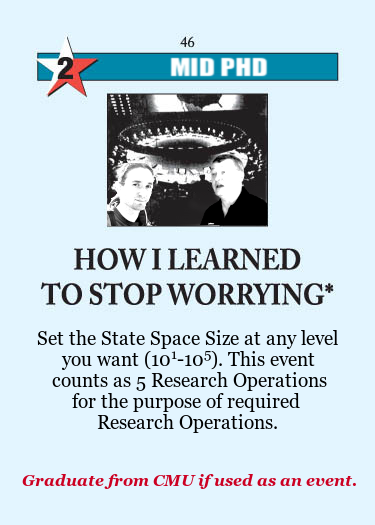
\includegraphics[width=0.55\textwidth]{how-i-learned.png}
\end{tabular}
\end{center}
